\documentclass{beamer}

\usetheme[progressbar=frametitle]{metropolis}
%\setbeamertemplate{frame numering}{fraction}
\useinnertheme{metropolis}
\useoutertheme{metropolis}
\usefonttheme{metropolis}
\usecolortheme{spruce}
\setbeamercolor{background canvas}{bg=white}

\usepackage{listings}

%\definecolor{owngreen}{rgb}{.125,.5,.25}
%\usecolortheme[named=owngreen]{structure}
%\usecolortheme{wolverine}

\author{Jorge F., Leonidas G., Giordano A.}

\title{Lesson 2}
\subtitle{"Think Big"}

\institute{UTEC}
\date{}

\begin{document}

\begin{frame}
  \titlepage
\end{frame}


\section{Asymptotic analysis}

\begin{frame}{Overview}

  \begin{itemize}
    \item In 2019, Twitter users send more than 500,000 tweets every minute.
    \item In 2019, 8.1 billion internet users.
    \item In 2018, 2.375 billion monthly active users in Facebook.
  \end{itemize}

  How can we decide which algorithm is better?

  \begin{center}
    
\includegraphics[width=0.23\linewidth]{../img/scalability}

    \textbf{Scalability}
  \end{center}

\end{frame}


\begin{frame}{Definition}
  A method of defining the mathematical boundation of the run-time performance or space usage of programs. With this, we can estimate the running time or space usage as function of the input size. Particularly, the order of growth in time o space of one algorithm according to input size.

  Using the asymptotic analysis we can easily estimate:
  \begin{itemize}
    \item Average Case - $\Theta(n)$ Theta notation
    \item Best Case - $\Omega(n)$ Omega notation
    \item Worst Case - $O(n)$ Big oh notation
  \end{itemize}
\end{frame}


\begin{frame}{Big O Notation}
  The formal way to express the upper bound of an algorithm running time.
  
  \begin{itemize}
    \item Ommit lower terms.
    \item Ommit multiplicative constants.
    \item Start from a particular input size $(n_0)$
    \item Sometimes the constant factors makes a considerable difference.
  \end{itemize}

  \begin{center}
    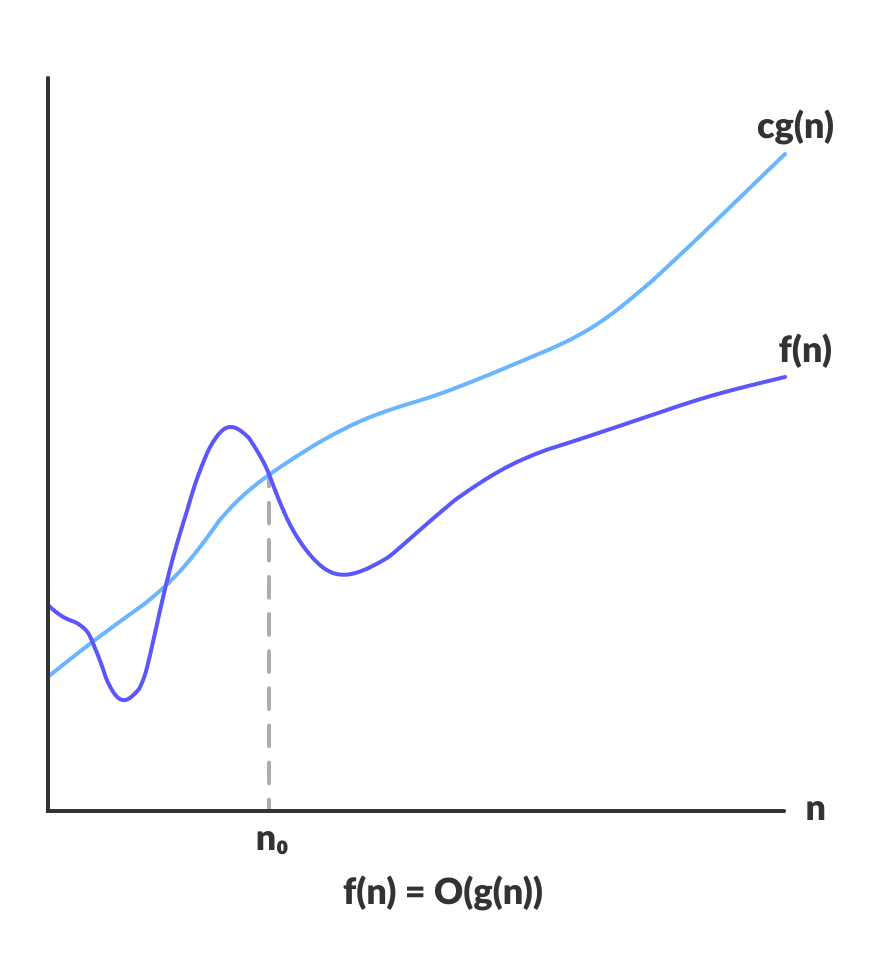
\includegraphics[width=.35\linewidth]{../img/bigO}
  \end{center}
\end{frame}


\begin{frame}{Space Usage vs Running Time}

  There exists almost always a \textbf{trade-off} in an algorithm between used space and run-time performance. Sometimes, we need to save computed values for future actions in order to improve the running time.

  \underline{Example}

  Fibonnaci Algorithm

\end{frame}

\begin{frame}{Simplification examples}

  \begin{itemize}
    \item Drop lower terms.
    \item Drop multiplicative constants.
  \end{itemize}

  \begin{center}

  $n^3 + n^2 + 1$

  $log(n) + n^2 + 100$

  $0.001*n^3 + 1$

  $ n*log(n) + n^2$

  $ n*log(n) + n + 10^{100}$

  $ n*log(n) + 500*n + 10^{100}$

  $ n*log(n) + n + 2^n$

  \end{center}

\end{frame}

\begin{frame}[fragile]{Examples Linear Algorithm}

  \begin{lstlisting}[language=C++]
    int main(){
      int ans=0;
      for(int i=0;i<100;i++){
        if(i%2==0)
          ans+=i;
      }
      cout<<ans<<endl;
      return 0;
    }
  \end{lstlisting}

\end{frame}

\begin{frame}[fragile]{Examples Quadratic Algorithm}

  \begin{lstlisting}[language=C++]
    int main(){
      int ans=0;
      for(int i=0;i<100;i++){
        for(int j=0;j<100;j++){
          if(i*i==j)
            ans+=i;
          if(j-i==i)
            ans-=i;
        }
      }
      cout<<ans<<endl;
      return 0;
    }
  \end{lstlisting}

\end{frame}

\begin{frame}{Examples of Time Complexity}
  \begin{center}
    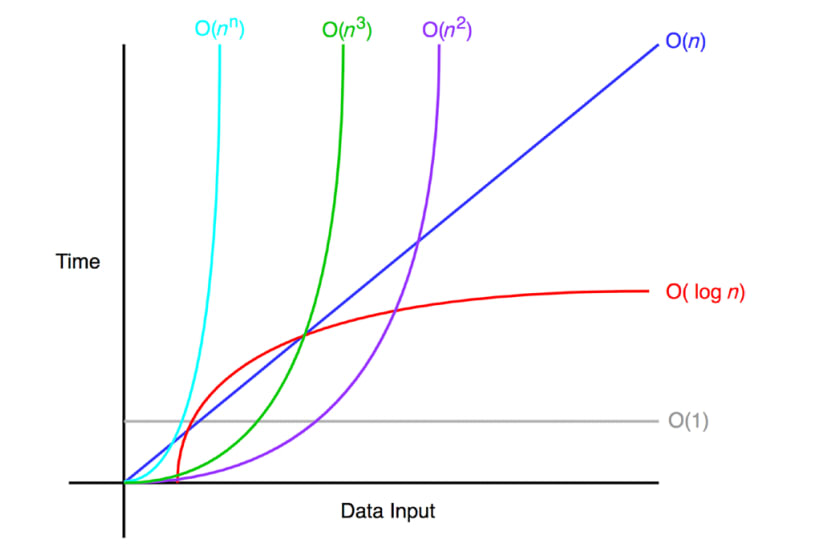
\includegraphics[width=.85\linewidth]{../img/bigOchart}
  \end{center}
\end{frame}

\iffalse
\begin{frame}{Programming Languages}

   \vspace{2mm}
   \begin{centering}
   \bgroup
   \def\arraystretch{5}
   \setlength\tabcolsep{35pt}.
   \begin{tabular}{ c c }
   
\includegraphics[width=0.23\linewidth]{../img/java} &
   
\includegraphics[width=0.23\linewidth]{../img/python} \\
   
\includegraphics[width=0.23\linewidth]{../img/kotlin} &
   
\includegraphics[width=0.23\linewidth]{../img/cpp}
   \end{tabular}
   \egroup
   \end{centering}

\end{frame}
\fi

\begin{frame}{Announcements}
\end{frame}

\end{document}
